\documentclass[12pt]{article}
\setlength{\textwidth}{17cm}
\setlength{\textheight}{24cm}
\setlength{\topmargin}{-2cm}
\setlength{\footskip}{1cm}
\setlength{\evensidemargin}{0cm}
\setlength{\oddsidemargin}{0cm}
\setlength{\parindent}{1cm}

\usepackage{allrunes}
\usepackage{amsmath}
\usepackage[magyar]{babel}
\usepackage[T1]{fontenc}
\usepackage[utf8]{inputenc}
\usepackage{fixltx2e}
\usepackage{multirow}
\usepackage{lmodern}

\usepackage[hyphens]{url}
\usepackage[unicode,colorlinks=true,breaklinks]{hyperref}
%\usepackage[dvips]{hyperref}
%should display links, but it does not work with \H accent
%and formulas in section titles

\hypersetup{colorlinks,linkcolor=blue,urlcolor=magenta,citecolor=magenta}
%Breaks long url`s in text, while keeping it one link:

\usepackage{amsfonts}
\usepackage{amsthm}
\usepackage{amssymb}


\theoremstyle{plain}
\usepackage{graphicx}

%\usepackage{gensymb}
\usepackage{float}

% For bra-ket notation
\usepackage{braket}

%% New commands
\newcommand{\dd}{\textrm{d}}

%% Pauli matrices
\newcommand{\sigx}{\sigma_x}
\newcommand{\sigy}{\sigma_y}
\newcommand{\sigz}{\sigma_z}

\newcommand{\paulix}{
    \left( \begin{array}{cc}
        0 & 1 \\
        1 & 0
    \end{array}
    \right)
}

\newcommand{\pauliy}{
    \left( \begin{array}{cc}
        0 & -i \\
        i & 0
    \end{array}
    \right)
}

\newcommand{\pauliz}{
    \left( \begin{array}{cc}
        1 & 0 \\
        0 & -1
    \end{array}
    \right)
}


\begin{document}
\title{10. tétel}
\author{Horváth Benedek}

\maketitle


\newpage
\begin{abstract}
    AD és DA konverterek – Digitális-analóg konverzió, AD-konverzió szukcesszív approximációval. A kvantálási zaj és a mintavételi törvény. Digitális jelek tömörítési módszerei: delta-moduláció és delta-szigma moduláció. Digitális számábrázolás és műveletvégzés.
\end{abstract}


Az anyag összegyűjtésekor legfőképpen Bagoly Zsolt Elektronika és méréstechnika előadásának a jegyzetét vettem alapul \cite{Bagoly}. Egyes témák leírásához Dülk Ivor BME-s oktató beágyazott rendszerekről szóló jegyzetét kivonatoltam \cite{BME}. Használtam még Dobos László hangfeldolgozásról szóló jegyzetét, ami a Digitális méréstechnika labor egy mérése volt \cite{hangfeldolgozas}, illetve egy Quora-cikket \cite{quora}. Amely fejezetek egyértelműen egy konkrét forrás gondolatmenetét követik, ott ezt a címben jelzem.


\section{Bevezetés}

A számítógépes rendszerek önmagukban csak számokat tudnak értelmezni és előállítani, a bemenő- és kimenőmennyiségeik mértékegység nélküli digitális értékek. A mérhető fizikai mennyiségek azonban túlnyomórészt folytonosak, és a mérőeszközök jelentős része analóg jelet ad ki magából. Ezért mielőtt bármilyen digitális jelfeldolgozási eljárást hajtanánk végre, a fizikai valóság releváns mennyiségeit szükségszerűen át kell alakítani a digitális rendszerek által értelmezhető számokká úgy, hogy a számok az eredeti mennyiségeket hűen tükrözzék. A másik oldalról pedig, a számítógép vezérelheti a külvilágot (mérőberendezést), jellemzően egy feszültségjellel. Ilyenkor tehát a digitális műveletek eredményeit kell valamilyen arányos módon visszaalakítani valódi fizikai mennyiséggé. Összességében tehát a digitális-analóg és az analóg-digitális irányú átalakítás egyaránt gyakori a mindennapokban. A legkézenfekvőbb, mindkét irányú konverziót tartalmazó hétköznapi példa a számítógépes hangrögzítés, tárolás, feldolgozás, illetve hangszórón történő lejátszás. Ezekre a feladatokra dedikált áramköri egységek, az analóg-digitális (analog digital converter, ADC) és digitális-analóg (digital analog converter, DAC) átalakítók szolgálnak. Az eszközök egyszerű vázlata \aref{fig:konverter_vazlat}. ábrán látható. 


\begin{figure}[H]
	\centering
	\begin{minipage}{0.47\textwidth}
		\centering
		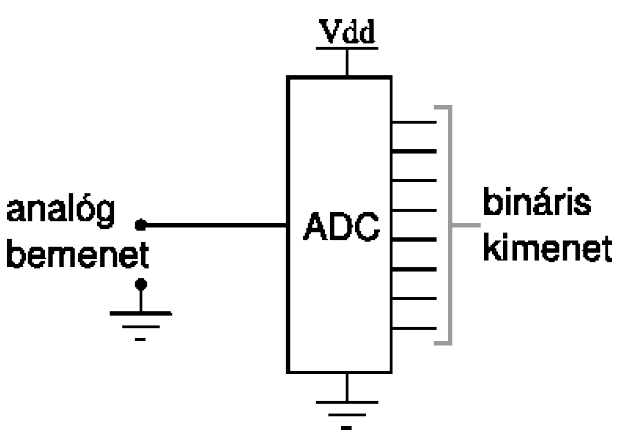
\includegraphics[width=1.0\textwidth]{./media/ADC_sketch.png}
	\end{minipage}\hfill
	\begin{minipage}{0.53\textwidth}
		\centering
		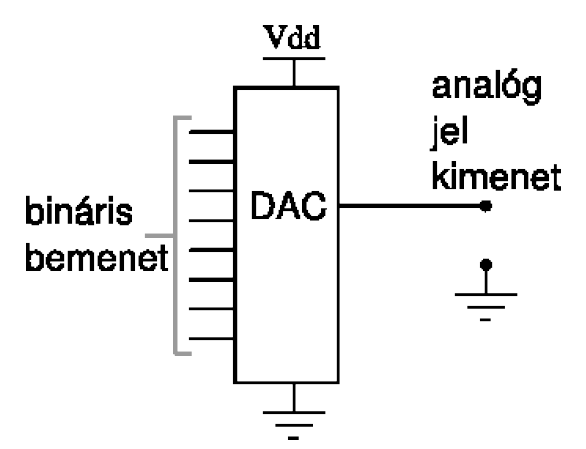
\includegraphics[width=0.85\textwidth]{./media/DAC_sketch.png}
	\end{minipage}
	\caption{Analóg-digitál (balra) és digitál-analóg (jobbra) konverter általános vázlata \cite{Bagoly}.}
	\label{fig:konverter_vazlat}
\end{figure}



\section{Digitális-analóg konverterek}

A digitális-analóg átalakítók (D/A konverterek) digitális jelek folytonossá alakítására használatosak. A D/A átalakítónak mind a bementi értéke, mind a kimeneti értéke az értékkészletében kvantált\footnote{Meg kell jegyezni, hogy ez az analóg oldalon természetesen csak elvileg igaz; a kimeneten fizikailag ténylegesen megjelenő feszültségérték időben folytonos. Nagy kvantumlépcső vagy alacsony mintavételi frekvencia esetén a kimeneti jelalak erősen torzított lesz az eredetihez képest, a felharmonikus tartalma igen magassá válik. Ennek jelentőségéről később ejtünk szót.}. A konverzió során valamilyen referenciafeszültség alapján áll elő a digitális értékeknek megfelelő analóg feszültség. A kimeneti feszültségtartományra az FSR (\textit{full scale range}) jelölést használva $q = FSR/2^n$ a felbontás (kvantumnagyság), azaz két diszkrét kimenet közti különbség, ahol $n$ a bitek száma a digitális reprezentációban. A bitek közt kitüntetett a legnagyobb, illetve legkisebb helyiértékű, ezeket MSB (\textit{most significant bit}) illetve LSB (\textit{least significant bit}) rövidítéssel illetjük.
Az alábbiakban két egyszerű elektronikai megvalósítását nézzük meg a digitális-analóg átalakítóknak.


\subsection{Bináris súlyozású DAC \cite{Bagoly}}

\Aref{fig:dacbinaris}. ábrán egy 6 bites bináris súlyozású D/A konverter látható.
Az $R_i$ ellenállások nagysága az egyes bitek helyiértékével fordítottan arányos, ezért a biteknek megfelelő $I_i$ áramok a helyiértékeknek megfelelően súlyozódnak. A csomópontban az egyes bitek összegződnek, így a bináris bemenettel arányos $\sum_i I_i$ áram jelenik meg.
A műveleti erősítő kimenetén az áramok összegével arányos $U = - R_{visszacsatolás} \sum_i I_i$ feszültség jelenik meg. A kimeneti tartomány nagysága az $R_{visszacsatolás}$ ellenállással állítható be.
Meg kell jegyezni, hogy az egyes bitekhez tartozó $V_i$ bemenő feszültségek digitális kapuk kimenetei, azaz értékük közel 0 vagy az $U_T$ tápfeszültség. A kapuk kimenő feszültségének a DAC felbontásán belül meg kell egyezni, máskülönben az átalakítás nem pontos. A bináris súlyozású átalakító ugyan egyszerű felépítésű, az ellenállások széles skálán mozgó értéke a bitszámmal növekvő hátrányokkal is jár: a nagy ellenállások véges pontossága kedvezőtlenül növelheti a konverziós hibát (pl. 10 bit esetén az $MSB=512$ 10\%-os hibája 5 $LSB$-nyi hibát jelent), noha a bitszám növelése a felbontást lenne hívatott növelni. Ezen túlmenően a különleges ellenállások előállítása is költséges.


\begin{figure}
	\centering
	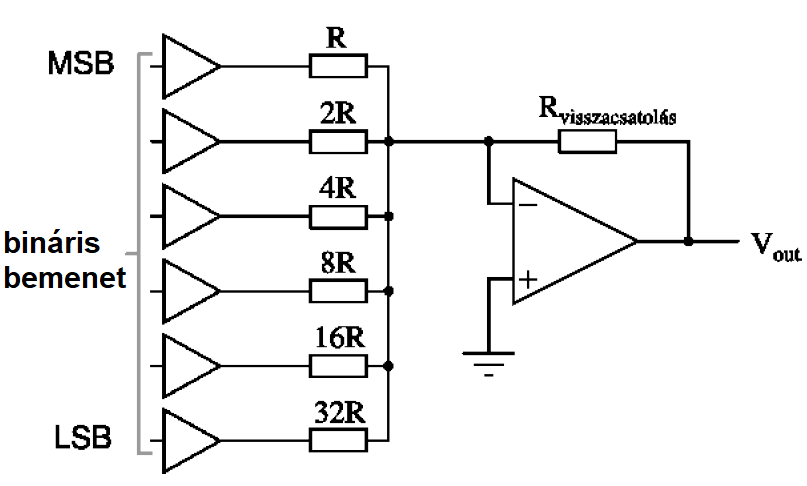
\includegraphics[width=0.7\linewidth]{media/DAC_binaris}
	\caption{6 bites bináris súlyozású digitális-analóg konverter áramköri vázlata \cite{Bagoly}.}
	\label{fig:dacbinaris}
\end{figure}


\subsection{R/2R létra \cite{Bagoly}}

A bináris súlyozású DAC problémáit hatékonyan küszöböli ki a beszédesen R/2R létrának nevezett kapcsolás, ami \aref{fig:dacletra}. ábrán látható.
A bitek bináris súlyozása különböző ellenállások helyett egy speciális kapcsolással valósul meg, mindössze kétféle ellenállás használatával. A kapcsolást áttekintve, a Kirchoff-egyenleteket felírva belátható, hogy a műveleti erősítő bemenetén lévő létraáramkör a feszültségeket a bitek helyiértékével súlyozva összegzi, MSB-től kezdődően $U_0/2$, $U_0/4$, $U_0/8$ stb. járulékok adódnak hozzá az összegzéshez.


\begin{figure}
	\centering
	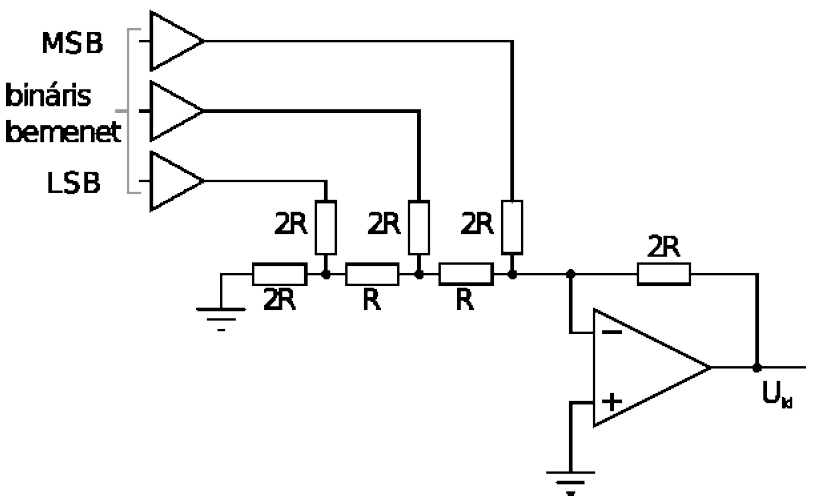
\includegraphics[width=0.7\linewidth]{media/DAC_letra}
	\caption{3 bites R/2R létra típusú digitális-analóg konverter kapcsolási rajza \cite{Bagoly}.}
	\label{fig:dacletra}
\end{figure}


\section{Analóg-digitális konverterek}

Az analóg-digitális átalakítók a bemenetükre kapcsolt folytonos, analóg jelet egy órajel-generátor által meghatározott mintavételezési frekvencia szerint bináris számértékekké alakítják. Az áramkör kimenetén a jel feszültségszintjének digitális reprezentációja jelenik meg. Az A/D átalakítók általában a gyártó által előre meghatározott feszültségtartomány digitalizálására képesek, így a jel feszültségszintjét megfelelő analóg áramkörrel kell illeszteni az A/D konverter bemenetéhez. Az esetek többségében unipoláris A/D konvertereket alkalmaznak, amelyeknél a jeltartomány egyik széle általában a nulla, a méréshatár szélét végértéknek (Full Scale, FS) jelölik. A bipoláris pozitív-negatív átalakítók általában valamilyen szinteltolást alkalmaznak a bemeneten: a mérhető jeltartomány így közrefogja a nulla értéket, és általában szimmetrikus (FSR, Full Scale Range). Az átalakítók általában lineáris karakterisztikájúak, azaz a digitálisan megkülönböztetett szintek között egyenlő lépésközök vannak a bemenő analóg feszültségben. Egy ADC felbontóképességének azt az analóg jelváltozás nevezzük, ahol a kimenet vált, azaz ahol a változás megkülönböztethető a digitális kimeneten is. A felbontóképesség egy $n$ bites bináris kódolású konverter esetén elvileg megegyezik a $q = FSR/2^n$ kvantumnagysággal, ahol $2^n$ a konverter lehetséges digitális kimeneteinek száma. A felbontóképességet általában bitekben adják meg, pl. 8, 10, 12,
16 stb. bites típusok vannak forgalomban. Az alábbiakban az A/D konverterek néhány gyakori típusát (elektronikai megvalósítását) vizsgáljuk meg.


\subsection{Szimultán (flash) A/D konverter \cite{Bagoly}}

\begin{figure}[]
	\centering
	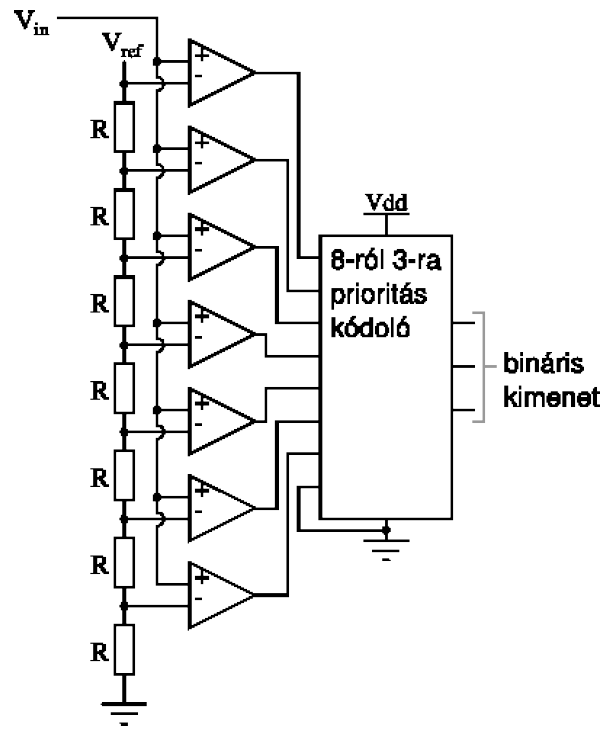
\includegraphics[width=0.5\linewidth]{media/ADC_flash}
	\caption{3 bites párhuzamos (flash) A/D konverter vázlata \cite{Bagoly}.}
	\label{fig:adcflash}
\end{figure}

\Aref{fig:adcflash}. ábrán egy $n=3$ bites szimultán ADC áramkört láthatunk. A megvalósításához a digitális szintek számánál 1-gyel kevesebb, azaz jelen esetben $2^n - 1 = 7$ db azonos ellenállásra van szükség, amelyek sorosan kapcsolva egyenlően osztják a referenciafeszültséget. Így az egyes ellenállások közti csomópontokban (a földhöz képest) a digitális szinteknek megfelelő feszültségek állnak elő. A bemenő $V_{in}$ analóg jelet komparátorok sorozata hasonlítja össze az ellenálláslánc $V_{ref}$-ből osztott referenciafeszültségeivel. Amennyiben a komparátor pozitív bemenetére kötött bemenő jel nagyobb a negatívra kötött referenciafeszültségnél, a kimenet logikai 1, ellenkező esetben 0. A komparátorok kimenetét egy kódoló áramkör alakítja át bináris jellé. A kimeneten végeredményül a legmagasabb logikai 1-et tartalmazó bemenet bináris címét kapjuk, azaz a bemenő feszültséget bináris értékké konvertálva. A kódoló áramkör felépíthető kizáró-vagy kapuk és diódás logika felhasználásával, ennek technikai részleteire itt nem térünk ki. A flash konverter a leggyorsabb ADC, mivel az átalakítás egy órajel alatt megtörténik, sok egyéb típustól eltérően (lásd később). További érdekes tulajdonsága a flash konverternek, hogy a digitalizálási szintek csak az ellenálláslánctól függenek, azaz igény esetén nemlineáris skálát is lehet alkalmazni az analóg-digitális átalakításnál az ellenállások megváltoztatásával.



\subsection{Számláló A/D konverter \cite{Bagoly}}

\begin{figure}[]
	\centering
	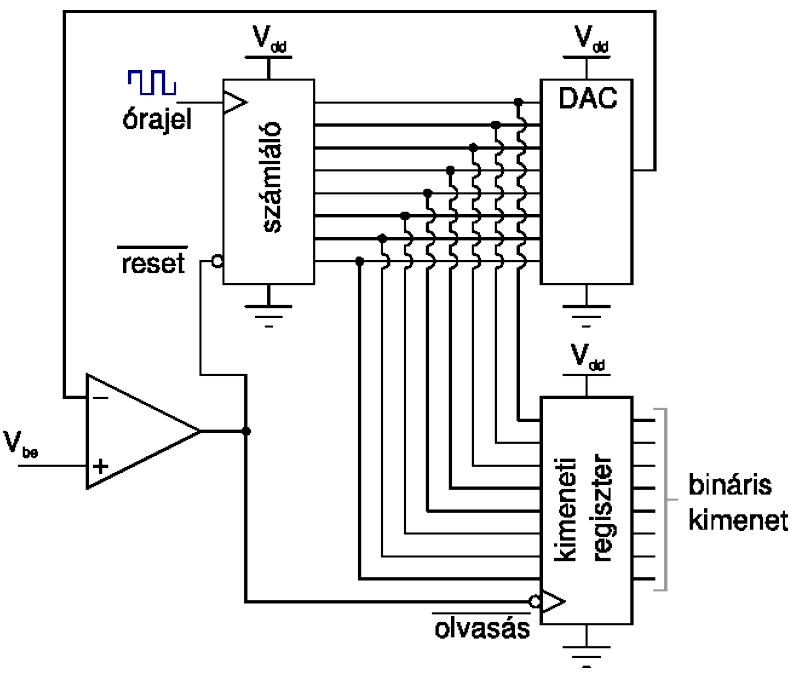
\includegraphics[width=0.7\linewidth]{media/ADC_szamlalo}
	\caption{8 bites számláló A/D konverter vázlata \cite{Bagoly}.}
	\label{fig:adcszamlalo}
\end{figure}

A számláló A/D konverter az egyik legegyszerűbb átalakító, vázlatát \aref{fig:adcszamlalo}. ábra mutatja. A berendezés "lelke" egy órajellel vezérelt bináris impulzusszámláló. Ennek kimenetét minden órajelkor egy D/A (!) konverterre vezetjük, ami egy nagy pontosságú $V_{ref}$ feszültségforrásból a számláló értékével arányos analóg feszültséget állít elő. Ezt egy komparátor segítségével összehasonlítjuk a bemenő, mérni kívánt ismeretlen $V_{be}$ analóg jellel. Amikor a DAC kimenő feszültsége eléri a $V_{be}$ feszültséget, akkor a komparátor átbillen, és ez egyrészt beírja a számláló értékét a kimeneti regiszterbe (pl. D tárolókból építhetünk ilyet), másrészt nullázza a számlálót. A mérés során tehát a mérendő értékkel arányos számú impulzus kerül a számlálóba, a mért érték digitális formában rendelkezésre áll. 
A konverter nagy hibája, hogy a mérési (átalakítási) idő függ a mérendő feszültségtől (lásd: \ref{fig:adcszamlalojel}. ábra). Ez az ingadozás a számítógépes jelfeldolgozást (pl. teljesítményspektrum meghatározása) bonyolítja, a digitális szűrést pedig megakadályozza. Gyorsan változó jelek mérésére nem alkalmas.


\begin{figure}[H]
	\centering
	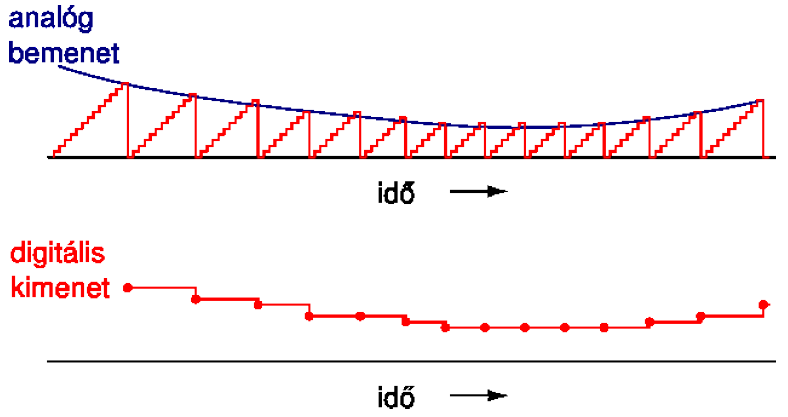
\includegraphics[width=0.7\linewidth]{media/ADC_szamlalo_jel}
	\caption{Számláló A/D konverterrel végzett konverzió szemléltetése. Jól látható a diszkrét lépések számának és az átalakítandó analóg feszültség nagyságának viszonya, illetve a konverzió közti időlépések különbözősége \cite{Bagoly}.}
	\label{fig:adcszamlalojel}
\end{figure}


\subsection{Szukcesszív approximációs A/D konverter \cite{Bagoly}}

\begin{figure}[]
	\centering
	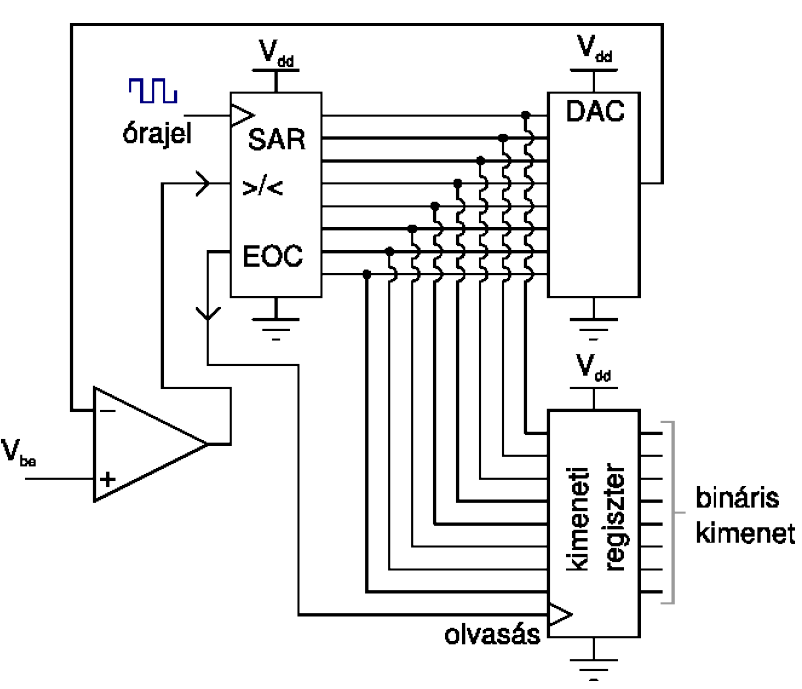
\includegraphics[width=0.7\linewidth]{media/ADC_SAR}
	\caption{8 bites szukcesszív approximációs A/D konverter vázlata \cite{Bagoly}.}
	\label{fig:adcsar}
\end{figure}


A szukcesszív approximációs konverter felépítésében és működésében hasonló a számláló A/D konverterhez, azonban annál összetettebb és hatékonyabb. A konverziót egy központi vezérlőlogika irányítja. A számláló helyett szukcesszív approximációs regiszter (SAR) található az áramkörben. A konverzió első lépéseként a SAR legnagyobb helyiértékű bitje (MSB) logikai 1-be billen, míg az összes többi 0 marad. Ebből a számláló A/D átalakítóban is látott DAC egység analóg jelet állít elő, ami épp a mérési tartomány ($V_{ref}$) fele. Ezzel a referenciajellel hasonlítja össze a $V_{be}$ mérendő analóg jelet a komparátor. Amennyiben MSB-nél nagyobbnak bizonyul a konvertálandó analóg jel\footnote{Az MSB rövidítés egyaránt utalhat szó szerint egy bináris szám legnagyobb helyiértékű bitjére, annak decimális értékére, illetve az ennek megfelelő nagyságú analóggá konvertált feszültségre.}, a bit értéke 1 marad, ellenkező esetben a vezérlő SAR törli a bitet. Ezáltal kiderül, hogy a mérési tartománynak melyik felébe esik a mérendő jel. 
A további órajelek során a SAR a bináris számrendszer csökkenő helyértékeinek megfelelő biteknél megismétli az előbbi eljárást, miközben a korábban beállított nagyobb helyiértékű bitek változatlanok maradnak. Egy ciklusban tehát mindig feleződik az előző lépésben vizsgált mérési tartomány. A komparátor megvizsgálja, hogy a mérendő mennyiség kisebb vagy nagyobb-e, mint az aktuális mérési tartomány fele: a bit értéke ennek megfelelően áll be. A legkisebb helyiértékű bit (LSB) meghatározása után a SAR a bemenő analóg jel digitális értékét tartalmazza (a konverzió pontossága LSB).\footnote{Tekintsünk egy konkrét példát: 13.7~V analóg jel esetén egy 5 bites konverternél $MSB=16$, ez tehát 0-nak adódik. A 32~V-ig terjedő mérési tartománynak mostantól az alsó felét vizsgáljuk. A következő helyiérték már 1, mivel $13.7>8$, tehát 8 és 16 közé szűkült a vizsgálandó tartomány. Így tovább, mivel $8+4<13.7$, $8+4+2>13.7$, $8+4+1<13.7$, a bitek értéke sorban, azaz a bináris szám: 01101. A mérés értéke 13~V-nak adódik, a tizedesjegy csonkolódik, mivel $13.7<14$. 0.7~V a konverziós hiba.}
A konverzió végét az áramkör jelzi (EOC, \textit{end of conversion}), és a kimeneti regiszter ekkor olvassa be a SAR bitjeit. A következő átalakítást a külső áramkör a SAR törlésével indítja.
Figyelemre méltó, hogy a mérési idő a SAR regiszter méretétől, azaz a konverter felbontásától függ, mivel az összehasonlítások száma megegyezik a AD bitjeinek számával (pl. 8 bit esetén 8 ciklus kell a teljes méréshez); a számláló A/D konverterrel ellentétben a konverziós idő a mérendő jel értékétől független. Megemlítendő még, hogy a szukcesszív approximációs ADC működtetéséhez szükség van gyors mintavevő és jelnyújtó (\textit{sample and hold}) áramköri egységekre annak érdekében, hogy a szukcesszív approximáció több órajeles időtartama alatt stabil legyen a konvertált mennyiség. Összességében a szukcesszív approximációs A/D konverter az egyik legelterjedtebb átalakító a számítógépes mérésadatgyűjtő berendezésekben, viszonylag egyszerű felépítése, pontossága és a legtöbb gyakorlati alkalmazáshoz kellőképpen gyors sebessége miatt.



\section{Mintavételi törvény}

A gyakorlatban mindennapos, hogy időben gyorsan változó analóg jeleket kell digitálissá konvertálni (mérni). Ilyenkor fontos, hogy az A/D átalakítási frekvencia (conversion rate, $f_cr$) kellőképpen magas legyen, ami egyben általában magas jelmintavételi frekvenciát ($f_m$) és rövid mintavételi periódusidőt ($T_m$) is jelent. Közönséges átalakítóknál a mintavétel ritkábban történik, mint a konverzió, de egyes nagy sebességű átalakítóknál (pl. digitális oszcilloszkóp) a tényleges mintavételek közti idő akár rövidebb is lehet a konverziós időnél (ami megfelelő jeltartó elektronikával lehetséges).
Az ADC szakaszos működése megköveteli, hogy a bemenő jel ne változzon a $T_m$ mintavételi időnél gyorsabban. Ellenkező esetben jelentősen torzul a mérés. Erre egy egyszerű szemléltetés látható \aref{fig:mintavetelintuitiv}. ábrán.


\begin{figure}
	\centering
	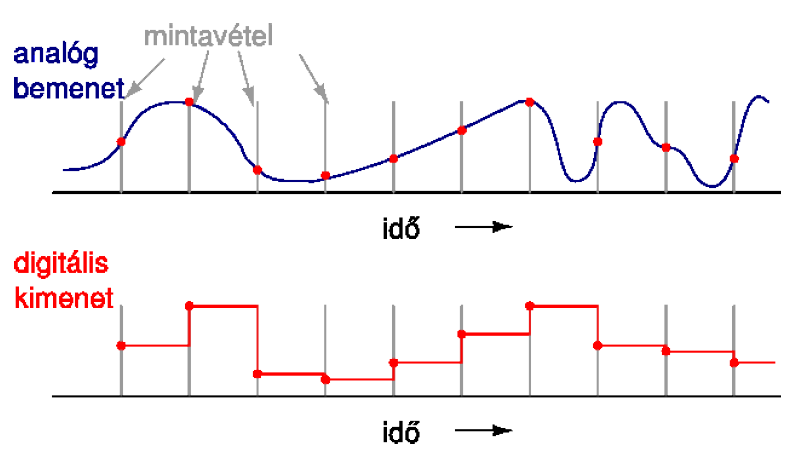
\includegraphics[width=0.7\linewidth]{media/mintavetel_intuitiv}
	\caption{Időben változó jel alulmintavételezésének egyszerű illusztrációja \cite{Bagoly}.}
	\label{fig:mintavetelintuitiv}
\end{figure}


Intuitíve is belátható, hogy időben változó jel konverziója során a jel legmagasabb frekvenciájú összetevőjéből is periódusonként legalább két mintát kell venni. Ezt mondja ki a Nyquist-Shannon-féle mintavételi törvény: egy $f$ frekvenciájú
tisztán szinuszos jel digitális reprezentációjához legalább $2 \cdot f$ frekvenciával szükséges mintavételezést végezni. Tetszőleges változó jelre tehát

\begin{equation}
	2 \cdot f_{max} \leq f_m,
\end{equation}
ahol $f_{max}$ a legnagyobb frekvenciájú komponens, $f_m$ a mintavételezési frekvencia. Az $f_{max}$ frekvenciát, ami tehát a legnagyobb, még a mintavételezett adatsorból visszaállítható frekvencia, Nyquist-frekvenciának is szokták hívni.
Mivel az analóg jelek általában nem mentesek a mintavételezési frekvenciánál nagyobb frekvenciájú komponensektől (felharmonikusok), ezért az A/D konverterek bemenetét aluláteresztő szűrőn keresztül kell meghajtani. Ha ezt nem tennénk meg, akkor a mintavételezett jel jelentősen torzulna. A mintavételi törvény precíz matematikai megfogalmazása a Nyquist-Shannon-tétel: egy olyan függvényt, ami nem tartalmaz
egy adott $f_{max}$ feletti Fourier-komponenseket, egyértelműen meghatároz egy
olyan számsor, ami a függvény értéke $\frac{1}{2 \cdot f_{max}}$ távolságú pontokban mérve.



\section{Kvantálási zaj \cite{BME}}

Egy A/D konverter jellegéből adódóan a folytonos analóg jel diszkrét digitális jellé való átalakítása során fellép a kvantálási hiba: a bemenő analóg érték és az eredményül kapott digitális érték különbsége. Ez csonkolásos esetben $LSB$-ig terjed, kerekítéses konverziónál $\pm LSB/2$ nagyságú. Ez egy elvi érték a konverzió hibájára: valójában sok egyéb áramköri tényezőből adódóan különféle, általában nagyobb mértékű hibák adódhatnak ezen kívül. A digitális jelfeldolgozás szempontjából a kvantálási hibának komoly jelentősége van. Gyakori feltételezés, hogy additív zajnak tekintjük, aminek értéke független a bemenő jeltől. A konvertált jel így az eredeti jel és a kvantálási zaj összege:
\begin{equation}
	U_{AD} (t) = U(t) + n_q (t),
	\label{eq:kvant_zaj}
\end{equation}
ahol $U_{AD}$ az A/D konverzió eredménye, $U$ a bemenő analóg jel, $n_q$ a jeltől függetlennek feltételezett kvantálási zaj. A függetlenség elvi szinten természetesen nem igaz, hiszen a jelből determinisztikusan származik a kvantálási hiba, az azonban általában helytálló feltételezés, hogy a hiba jelalakja nem korrelál a jellel. A kvantálási zajra vonatkozóan általában azt is feltesszük, hogy egyenletes az eloszlása a [$-LSB/2$, $LSB/2$] intervallumban, azaz fűrészjel (lásd: \ref{fig:kvantalasihiba}. ábra). Az egyenletes eloszlás és a korrelálatlanság a bitszám (felbontás) növelésével jobban teljesül. Egyenletes eloszlást feltételezve, a kvantálási zaj teljesítménye (varianciája):
\begin{equation}
	\sigma^2 (n_q) = \int_{-\frac{q}{2}}^{\frac{q}{2}} \left( \braket{n_q} - n_q \right)^2 f(n_q) \dd n_q = 
	\int_{-\frac{q}{2}}^{\frac{q}{2}} n_q^2 \frac{1}{q} \dd n_q = 
	\frac{1}{3q} \left[ n_q^3 \right]_{-\frac{q}{2}}^{\frac{q}{2}} = \frac{q^2}{12},
	\label{eq:zaj_power}
\end{equation}
ahol $q$ a kvantumnagyság; a zaj várható értéke 0, $f(n_q) = \frac{1}{q}$ a konstans sűrűségfüggvény. 
Tegyük fel továbbá, hogy a kvantálási zaj a teljes Nyquist-sávszélességben, azaz 0 Hz-től a mintavételi frekvencia feléig ($f_m/2$) jelen van, és teljesítménye a teljes spektrumban egyenletesen oszlik el. Ez a kvantálási zaj fehérzajmodellje. A Fourier-transzformáció linearitása miatt elmondható az is, hogy a konvertált jel spektruma az eredeti jel spektrumának és a kvantálási hiba spektrumának az összege (vö. (\ref{eq:kvant_zaj})). Amennyiben egyetlen szinuszjelet tekintünk, annak spektruma egyetlen pontba koncentrálódik. $N$ pontban mintavételezett szinusz esetén a kvantálási zaj spektruma $N/2$ diszkrét pontba szóródik szét 0 és $f_m/2$ között, a fehérzajmodell szerint egyenletesen. Így a szinuszjel frekvenciáján a $N/2$-ed részére csökken a kvantálási zaj. Azonban egy probléma is adódhat a Fourier-transzformációs zajcsökkentésből: ha a $T$ szinuszperiódus a $T_m$ mintavételi időköz egész számú többszöröse -- azaz mindig ugyanazokban a fázisokban veszünk mintát a jelből --, a kvantálási zaj az alapharmonikus, a vizsgált szinuszjel frekvenciájának egész számú többszöröseinél összpontosul. Ez azt jelenti, hogy a zaj korrelál a jellel, ami ellentétben áll a fehérzajmodell alapfeltevésével. Ahhoz, hogy a zaj valóban korrelálatlan legyen a jellel, az szükséges, hogy a mérés során a mintaszám és mért periódusok száma relatív prímek legyenek \cite{BME}.


\begin{figure}
	\centering
	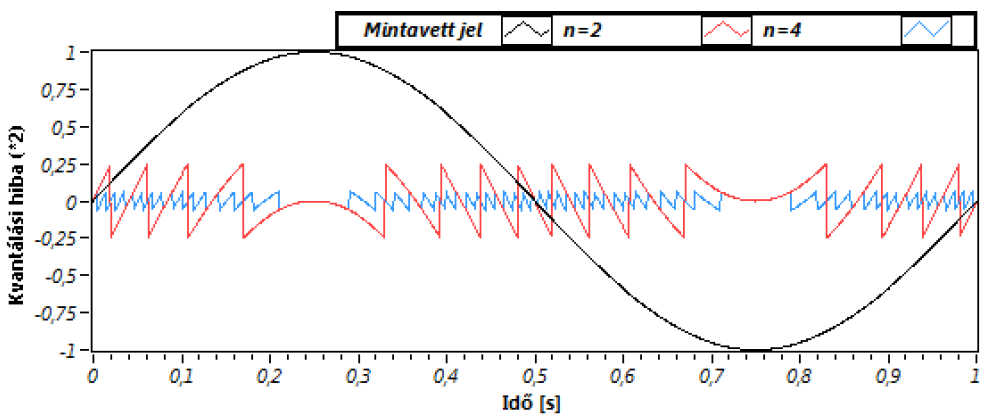
\includegraphics[width=1\linewidth]{media/kvantalasi_hiba}
	\caption{A kvantálási hiba időfüggése szinuszos analóg jel konverziója során 2, illetve 4 bit esetén. A jobb láthatóság érdekében a hibát kétszeres szorzóval mutatja az ábra \cite{BME}.}
	\label{fig:kvantalasihiba}
\end{figure}



\section{$\Delta$-$\Sigma$-moduláció \cite{BME}}

Az fentiekben ismertetett additív, fehér spektrumú kvantálási zajmodellt (\ref{eq:kvant_zaj}) alkalmazva, az átalakított jel spektruma a Fourier-transzformáció linearitása miatt az eredeti jel spektrumának és a kvantálási zaj (hiba) spektrumának az összege. A kvantálási zajról elmondható, hogy a teljesítménysűrűségének a spektruma egyenletesen oszlik el az $f_m/2$ frekvenciáig, és az általa határolt téglalap alatti terület $\frac{q}{\sqrt{12}}$ (vö. (\ref{eq:zaj_power})). Gondolatkísérletként növeljük most a mintavételi frekvenciát $k \cdot f_m$-re! Ez esetben 0 és $k \cdot f_m/2$ frekvencia között oszlik meg a teljesítményspektrum egyenletesen, a korábbihoz képest $k$-szor annyi pontban. Az alatta lévő terület viszont változatlanul $\frac{q}{\sqrt{12}}$, így egy pontban $k$-ad részére csökken a kvantálási zaj teljesítménye. Adott szinuszjel vizsgálatakor ez $k$-szoros jel-zaj arányt jelent.
Túlmintavételezéskor tehát az átalakító kvantálási hibájának egy szélesebb spektrumba való szétszórásával az adott jel konverziójakor bekövetkező kvantálási hiba csökkenthető, más szóval a felbontás növelhető. Ez effektíve olyan, mintha plusz biteket adnánk hozzá az A/D átalakítóhoz.

Az úgynevezett $\Sigma-\Delta$ átalakítók működése részben ezen az ötleten alapszik. A túlmintavételezés mellett jelentősen javítható a jel-zaj arány zajformálással: a kvantálási zajt olyan módon kell formálni, hogy a spektrumban a teljesítménye egyenletes eloszlás helyett a nagyfrekvenciás tartományba koncentrálódjon, és így a mérendő jel komponenseire kisebb legyen a zaj értéke. A zajformálásra szolgál a $\Sigma-\Delta$ modulátor. A zaj spektrumából (digitális) aluláteresztő szűrővel (LPF, \textit{low-pass filter}) kiszűrhető a nagy frekvenciába eső nagy teljesítményű régió, majd a frekvencia decimálásával $f_m$-re kell csökkenteni a már szűrt jel mintavételezési frekvenciáját, hogy az a digitális kimenet számára feldolgozható legyen. A $\Sigma-\Delta$ átalakító működését \aref{fig:sigmadeltaflowchart}. ábra foglalja össze. Az eszköz tehát intenzív digitális jelfeldolgozást hajt végre, ami igen számításigényes folyamat (pl. a sokszoros túlmintavételezés és a nagy adatmennyiség szűrése).


\begin{figure}
	\centering
	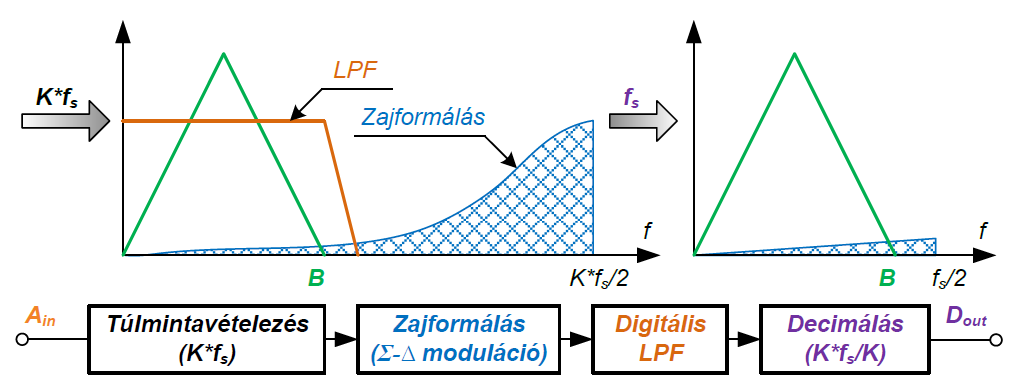
\includegraphics[width=1\linewidth]{media/sigma_delta_flowchart}
	\caption{$\Sigma-\Delta$ A/D konverter működésének vázlata és illusztrációja \cite{BME}.}
	\label{fig:sigmadeltaflowchart}
\end{figure}


A $\Sigma-\Delta$ modulátorban a bemenő analóg jel első lépésben egy különbségképzőre kerül, ami visszacsatolásos módszerrel a kvantálási hibát állítja elő. (A belső 1 bites A/D átalakító eredményét a visszacsatoló ágban lévő 1 bites (kétállapotú, $+U_{ref}$ vagy $ - U_{ref}$) D/A visszaalakítja
feszültséggé, majd a jelből kivonjuk a  1 bites D/A konverter kimenetét.) A különbségképző kimenetét (a kvantálási hibát) integráljuk, és az integrátor kimenetét digitalizáljuk az 1 bites A/D-vel. Ha az integrátor kimenete pozitív, akkor a komparátor kimenete logikai 1, egyébként logikai 0. Végeredményben a $\Sigma-\Delta$ modulátor kimenete egy digitális impulzussorozat, amiben a logikai nullák és egyesek egymáshoz képesti előfordulási aránya az eredeti analóg
bemenőjelnek a függvénye (lásd: \ref{fig:sigmadeltamodulator}. ábra).
Belátható, hogy a negatív visszacsatolás miatt a visszacsatolásban lévő D/A átalakító kimenőfeszültségének átlagértéke és így az eredményül kapott bitsorozat
átlagértéke is a bemenőjel átlagértékéhez tart, állandósult állapotban körülötte ingadozik. A bitsorozatot digitálisan szűrve, például átlagolva, az analóg jel értéke digitálisan előállítható, ugyanis a $\Sigma-\Delta$ modulációval a nagyfrekvenciás tartományba eltolt kvantálási zajnak a jelentős részétől megszabadulunk.


\begin{figure}
	\centering
	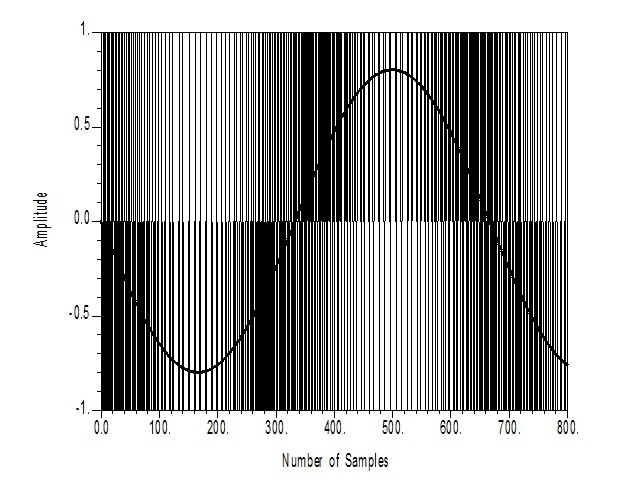
\includegraphics[width=0.5\linewidth]{media/sigma_delta_modulator}
	\caption{$\Sigma-\Delta$ modulátor analóg bemenete és a kvantáló kimenete \cite{quora}.}
	\label{fig:sigmadeltamodulator}
\end{figure}


\section{$\Delta$-moduláció \cite{quora}}

A $\Delta$-modulátor a $\Sigma-\Delta$-modulátorhoz hasonlóan negatív visszacsatoláson alapszik. Lényegében azt nézi, hogy az analóg jel a következő mintavételi ablakban alacsonyabb vagy magasabb, mint a konvertált digitális jel aktuális értéke. 1 bites esetben a következő forgatókönyv zajlik le: ha alacsonyabb az analóg jel az aktuális digitális értéknél, akkor 0-t ad ki a komparátor, és csökkentjük egy kvantálási lépcsővel a digitális jel értékét, ellenkező esetben az összehasonlítás eredménye logikai 1, és növeljük egy lépcsővel a digitális jelet. A mintavételi frekvencián kívül ez esetben a $q$ kvantumlépcső és a mérendő jel amplitúdója is meghatározó a konverzió sikeressége szempontjából: \aref{fig:deltamodulation}. ábra bal oldalán helyes, jobb oldalán hibás A/D átalakítást látunk $\Delta$-modulátorral. 


\begin{figure}[]
	\centering
	\begin{minipage}{0.47\textwidth}
		\centering
		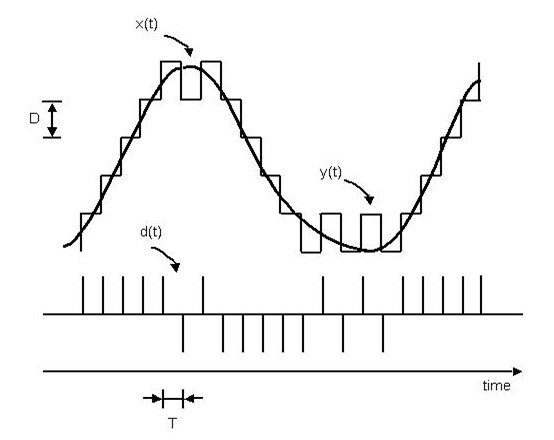
\includegraphics[width=1.0\textwidth]{./media/delta_modulation_correct.png}
	\end{minipage}\hfill
	\begin{minipage}{0.53\textwidth}
		\centering
		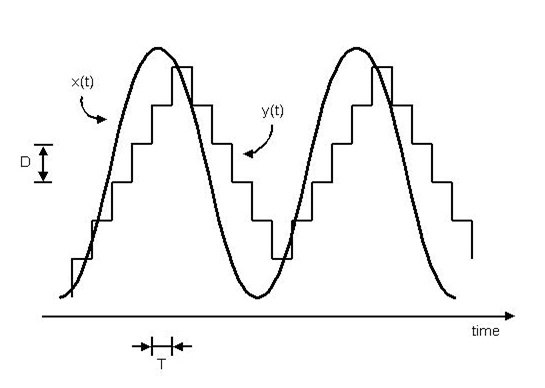
\includegraphics[width=1\textwidth]{./media/delta_modulation_incorrect.png}
	\end{minipage}
	\caption{$\Delta$-modulátor korrekt és hibás működésének illusztrációja \cite{quora}.}
	\label{fig:deltamodulation}
\end{figure}



\section{Digitális jelek tömörítése \cite{Bagoly}}

Egy eseményhalmaz megfigyelése során nyert átlagos információt, más szóval az adott eseményhalmaz entrópiája:

\begin{equation}
	H = - \sum_{i} p_i \log_2 p_i,
\end{equation}
ahol $i$ egy elemi esemény, $p_i$ annak valószínűsége. Például egy igen/nem döntés akkor jelenti a legnagyobb átlagos információmennyiséget, ha mindkét esemény bekövetkezése ugyanannyira valószínű ($p_i = 0.5$), más szóval, a jel zajszerű: ekkor az átlagos információ nagyságára $H = 1$-et kapunk \cite{Bagoly}. Ezt az információ-egységet hívják 1 bitnek. Amennyiben az események nem egyformán valószínűek (van valamiféle rendezettség), akkor az átlagos információmennyiség kisebb lesz. A rendezettség miatt pl. egy értelmes szöveg entrópiája kisebb egy vele azonos számú véletlen karakterből álló szövegénél, tömörítés nélkül mégis azonos adatmennyiséget jelentenek. Jól tömörített adathalmaz nem tartalmaz redundáns részt, a tömörített információ zajszerű. Másik hétköznapi példa egy videófelvétel: ez nem zajszerű, hiszen a szomszédos pixelek sokszor nagyon hasonlóak, és általában nem sokat változik a kép az előzőhöz képest. Ezeket a korrelációkat felhasználva különböző tömörítési eljárásokkal töredékére csökkenthető egy fájl, csökkentve az adatok átviteléhez szükséges időt és tárolásához szükséges memóriát. A tömörítés jóságának mérőszáma a kimenet entrópiája. Minél nagyobb az entrópia, annál inkább zajszerű a kimenet. A digitális tömörítési eljárásokat tekintve megkülönböztetünk veszteség nélküli és veszteséges módszereket: utóbbiak ugyan jobban tömörítenek, de az eredeti jelek tökéletes visszaállítása nem lehetséges a kimenetből, azonban a gyakorlatban általában megfelelő az eredmény. Veszteséges tömörítés pl. a jpeg és az mp3 kódolás: ezeket tipikusan az emberi érzékszervek működéséhez illesztik. Képek tömörítésénél az élek megtartása a legfontosabb, hangoknál a nagyobb amplitúdójú komponensek (a halk felharmonikusokat alig halljuk) \cite{Bagoly}.

Valójában a $\Delta$-moduláció is egy tömörítési eljárás: $n$ bites egymás utáni A/D konverzió eredményének (sok hasonló eredmény egymás mellett a folytonos bemenet miatt) eltárolása helyett a kiinduló állapotot és a rögzített kvantumlépcsőnyi nagyságú fel-le lépések sorozatát tároljuk. Ugyan a mintavételezési frekvenciát a $\Delta$-modulációhoz többszörösére kell növelni a hagyományos A/D konverzióhoz képest, a $\Delta$-modulációhoz akár 1 bit is elegendő, így a sávszélesség végeredményben csökkenthető. 

Hasonlóképp a $\Sigma-\Delta$ moduláció is tömörítéssel jár: itt is elegendő 1 bit, és a kvantálási zaj magas frekvenciájú régióba transzformálása és szűrése miatt szintén adatot eliminálunk.


\section{Digitális számábrázolás és műveletvégzés}

\subsection{Bináris számábrázolás}

A digitális memória alapegysége a bit, aminek két lehetséges értéke lehet: 0 vagy 1. A számábrázolás ezért kettes számrendszerben történik a digitális eszközökön: az egyes bitek 2 hatványainak megfelelő helyiértéket képviselnek, és minden 2-hatvány együtthatója 0-t vagy 1-et vehet fel. Egyszerű példaként tekintsük egy pozitív egész szám ábrázolását 8 biten (1 bájt)!

\begin{equation}
	107 = 0 \cdot 2^7 + 1 \cdot 2^6 + 1 \cdot 2^5 + 0 \cdot 2^4 + 1 \cdot 2^3 + 0 \cdot 2^2 + 1 \cdot 2^1 + 1 \cdot 2^0 \implies 01101011
\end{equation}
Törtek ábrázolására egy logikusan következő módszer a \textbf{fixpontos ábrázolás}: a bitek egy részét 2 negatív hatványainak dedikáljuk, így azok a törtrészt, a többi bit az egész részt reprezentálják. Például:

\begin{equation}
	13.25 = 1 \cdot 2^3 + 1 \cdot 2^2 + 0 \cdot 2^1 + 1 \cdot 2^0 +
	 0 \cdot 2^{-1} + 1 \cdot 2^{-2} + 0 \cdot 2^{-3} + 0 \cdot 2^{-4} 
	 \implies 1101.0100
\end{equation}
Ez a gyakorlatban nagyon nem praktikus, mert komolyan limitálja az ábrázolható számok nagyságát (a fenti példánál maradva, 8 helyett 4 egészrészbit esetén 255 helyett 15 lesz a legnagyobb ábrázolható egész szám), illetve egy rögzített felbontás alatt (itt: $2^{-4} = 0.0625$) nem lehet törtrészt ábrázolni. 


\subsection{Lebegőpontos számábrázolás}

\begin{figure}
	\centering
	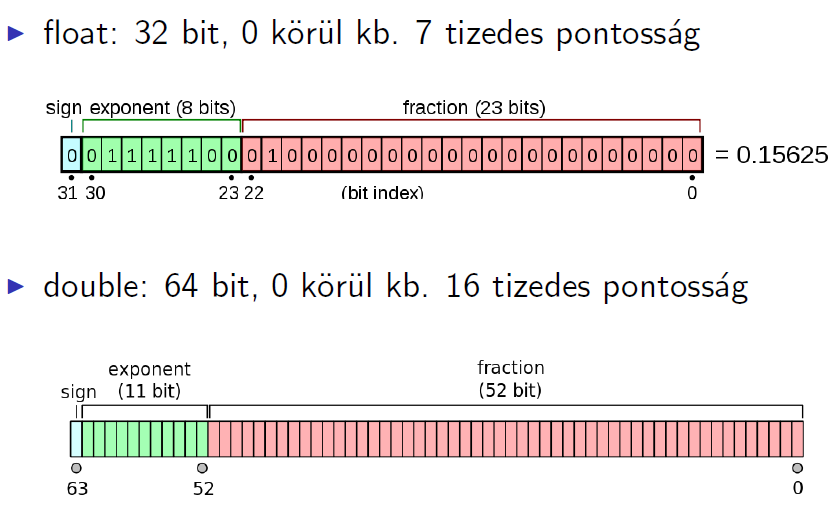
\includegraphics[width=\linewidth]{media/IEEE754}
	\caption{A szabványos 32 bites float és 64 bites double lebegőpontos számok bitkiosztása.}
	\label{fig:ieee754}
\end{figure}


A törtszámok digitális reprezentációjára a gyakorlatban \textbf{lebegőpontos számábrázolás}t használunk. Ennek motivációja a 10-es számrendszerben is használt normál alak:

\begin{equation}
	-2.3454612 \cdot 10^3, ~\mathrm{vagy} ~ -0.23454612E4.
\end{equation}
A számot itt három egységre bontottuk: előjel, mantissza és kitevő. A lebegőpontos számábrázolás hasonlót jelent a normál alakhoz, kettes számrendszerben. Egy számot az alábbi képlet szerint reprezentálunk digitálisan:

\begin{equation}
	(-1)^s \cdot f \cdot 2^{e-b},
\end{equation}
ahol $s$ az előjel (egyetlen bit, 0 vagy 1 egyértelműen meghatározza, hogy pozitív vagy negatív a szám), $f$ a mantissza, $e$ a kitevő (karakterisztika), $b$ pedig egy szabvány szerinti konstans. Az $f$, $e$ és $b$ mind 2-es számrendszerben reprezentált egész számok. A lebegőpontos számábrázolásra egyetlen hardveresen támogatott szabvány van, az IEEE 754. Ez alapján kétféle pontosság létezik: a 32 bites float és a 64 bites double. Ezek bitkiosztását és a $b$ konstans értékét lásd \aref{fig:ieee754}. ábrán. Az ábrázolás pontosságát a mantisszára kiosztott bitek határozzák meg: float esetében ez 7 tizedesjegyet jelent ($2^{23} \approx 10^6$, azaz 7 jegyű szám), double-nál 16-ot ($2^{52} \approx 10^{15}$, azaz 16 jegyű szám)\footnote{GPU-n létezik még a 16 bites half, ez tizes számrendszerben már csak 3-4 tizedesjegyre pontos, de bizonyos speciális esetekben ez elegendő.}. Megkülönböztetünk továbbá normált és nem normált lebegőpontos számokat. Normált számok esetében a mantissza teljesen "ki van töltve", a legnagyobb helyiértékén 1 áll, amit így nem is szükséges eltárolni. Ez az ábrázolás kihasználja az elérhető maximális pontosságot. Ezen kívül léteznek nem normalizált számok, amelyeknél a mantissza (törtrész) nagyobb helyiértékein 0 szerepel. Ezek kevésbé pontosak, azonban a normalizált számoknak van egy alsó limitje, aminél kisebb számok csak így ábrázolhatók.


\subsection{Műveletek lebegőpontos számokkal}

Az előbbiekben a statikus számábrázolás pontosságát vizsgáltuk meg. Fontos, hogy a műveletvégzés pontossága ettől jelentősen eltérhet.

\subsubsection{Összeadás, kivonás}

Ez a kritikus művelet. Ilyenkor a két számot azonos exponensre kell konvertálni (a nagyobb szám kitevőjére). A kisebb szám pontossága így csökken, hiszen kevesebb biten ábrázolódik (a nagyobb helyiértékeken 0 szerepel, nem normalizáltan ábrázolódik). Sok nagyságrend különbség esetén a műveletvégzési pontosság jelentősen romolhat az ábrázoláshoz képest.


\subsubsection{Szorzás, osztás}

Ezek a műveletek gyakorlatilag megtartják a pontosságot, akárhány nagyságrend különbség van a számok között. Ilyenkor a kitevőket összeadjuk/kivonjuk egymásból, a mantisszákat összeszorozzuk/elosztjuk egymással.



\bibliographystyle{plain}
\bibliography{references}

\end{document}
